\documentclass{article}
\usepackage[a4paper,margin=1cm,footskip=.5cm]{geometry}
\usepackage{amsmath,amssymb,amsthm,amsfonts,mdframed,kotex}
\newcounter{problem}
\newcommand{\bp}
{\stepcounter{problem}\begin{mdframed}
[frametitle={\theproblem},skipabove=10pt,skipbelow=10pt]}
\newcommand{\ep}{\end{mdframed}}
\newcommand{\parall}{\mathbin{\!/\mkern-5mu/\!}}
\title{미리-02:중등도형2}
\date{\today}
\author{}
\begin{document}
\maketitle
\newpage
\bp
\(AD\parall BC\)일 때
일 때 \(\triangle AOB=\triangle DOC\)를 증명하여라.
\par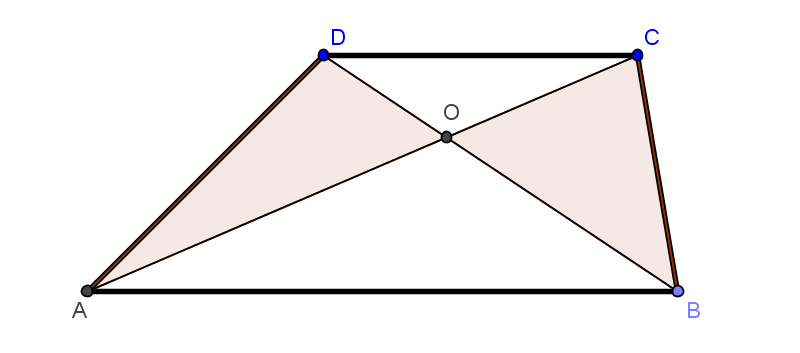
\includegraphics[width=0.5\textwidth]{advanced_geometry_30}
\ep

\bp
\(AE:EC=7:2\)일 때, \(\frac{PD}{AP}\)를 구하여라.
\par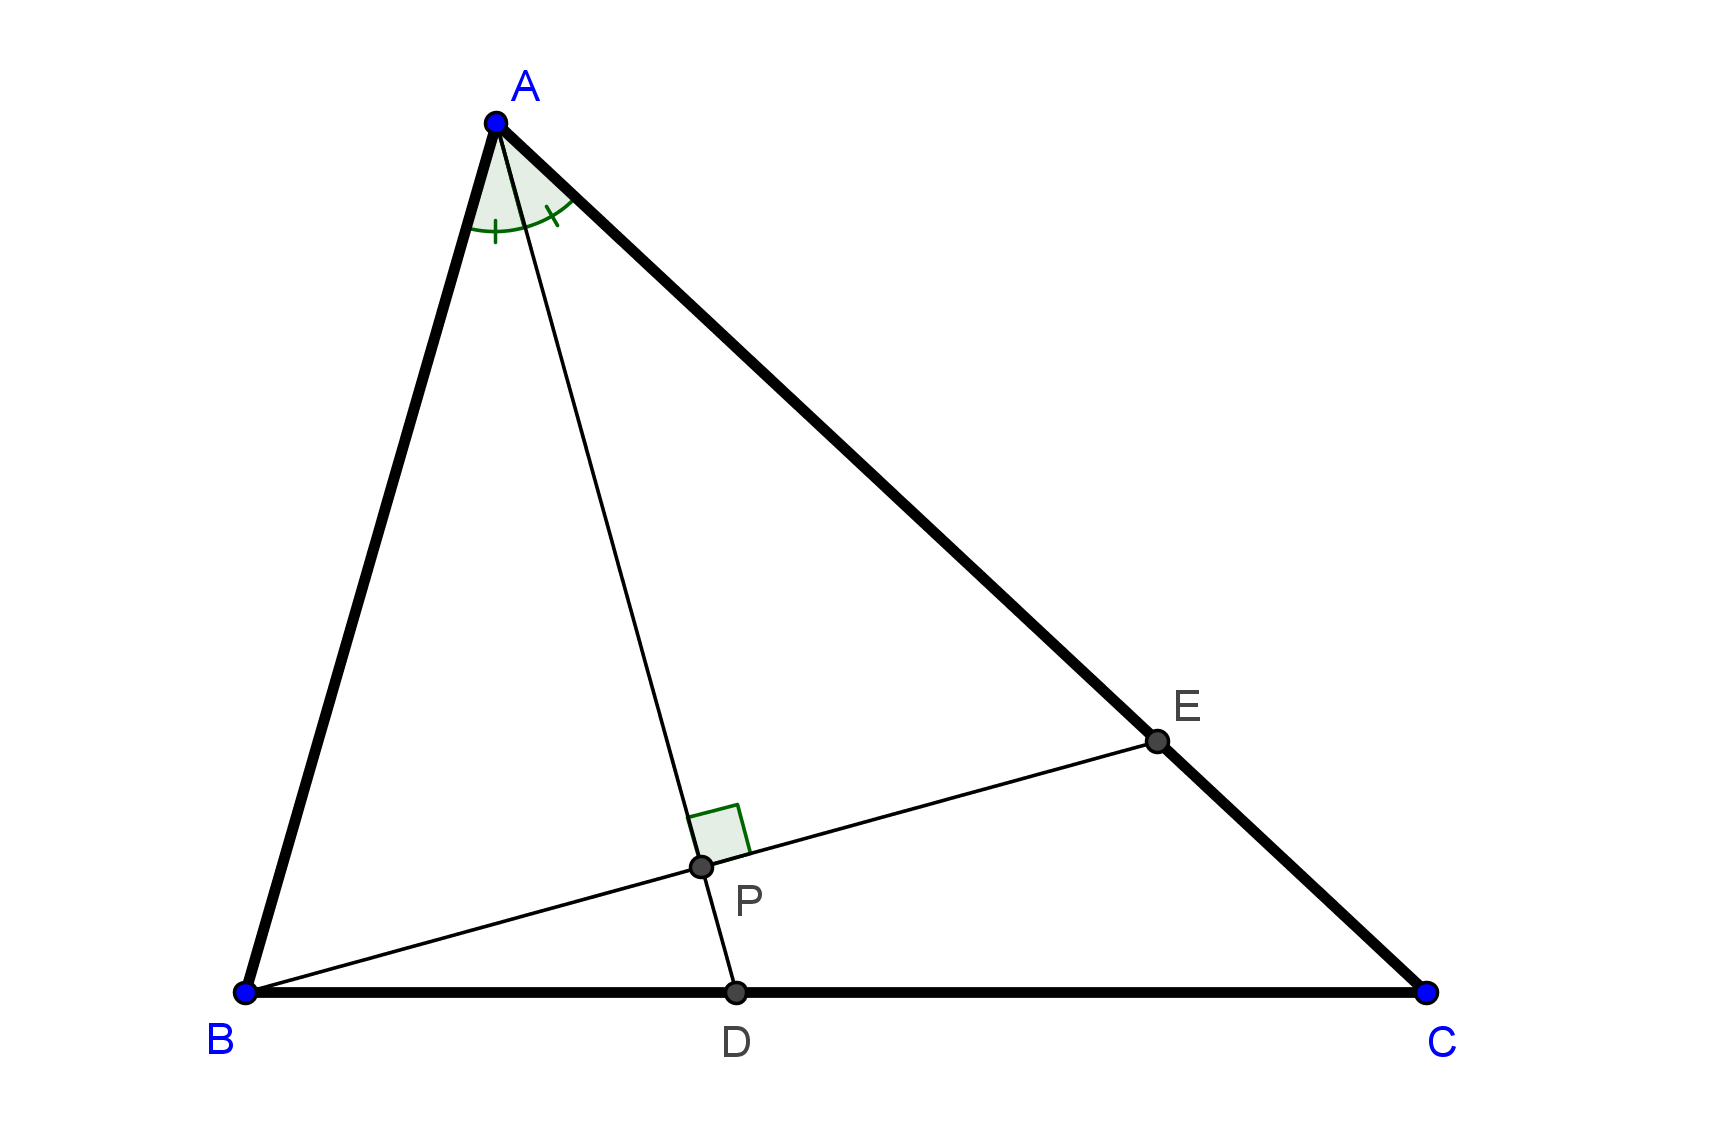
\includegraphics[width=0.5\textwidth]{advanced_geometry_55}
\ep

\bp
\(AC=3\), \(AE=2\), \(EB=6\), \(BD=9\)일 때 \(GF\)의 길이를 구하여라.
\par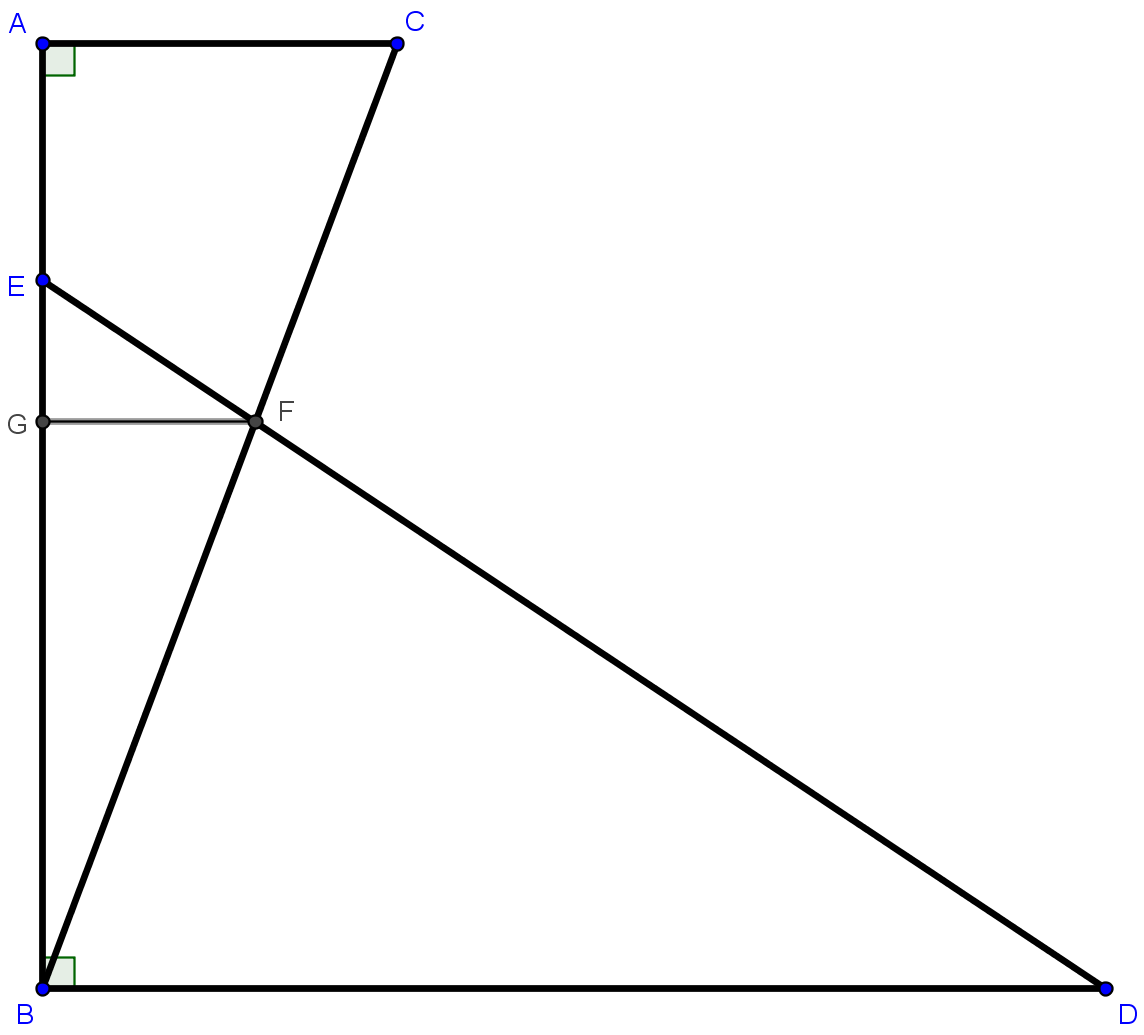
\includegraphics[width=0.5\textwidth]{advanced_geometry_65}
\ep

\pagebreak
\bp
\(\angle RPQ\)를 구하여라.
(그림에서 \(AB=CD\)이고 \(L\), \(M\), \(N\)은 각각 \(BC\), \(AD\), \(AC\)의 중점이다.)
\par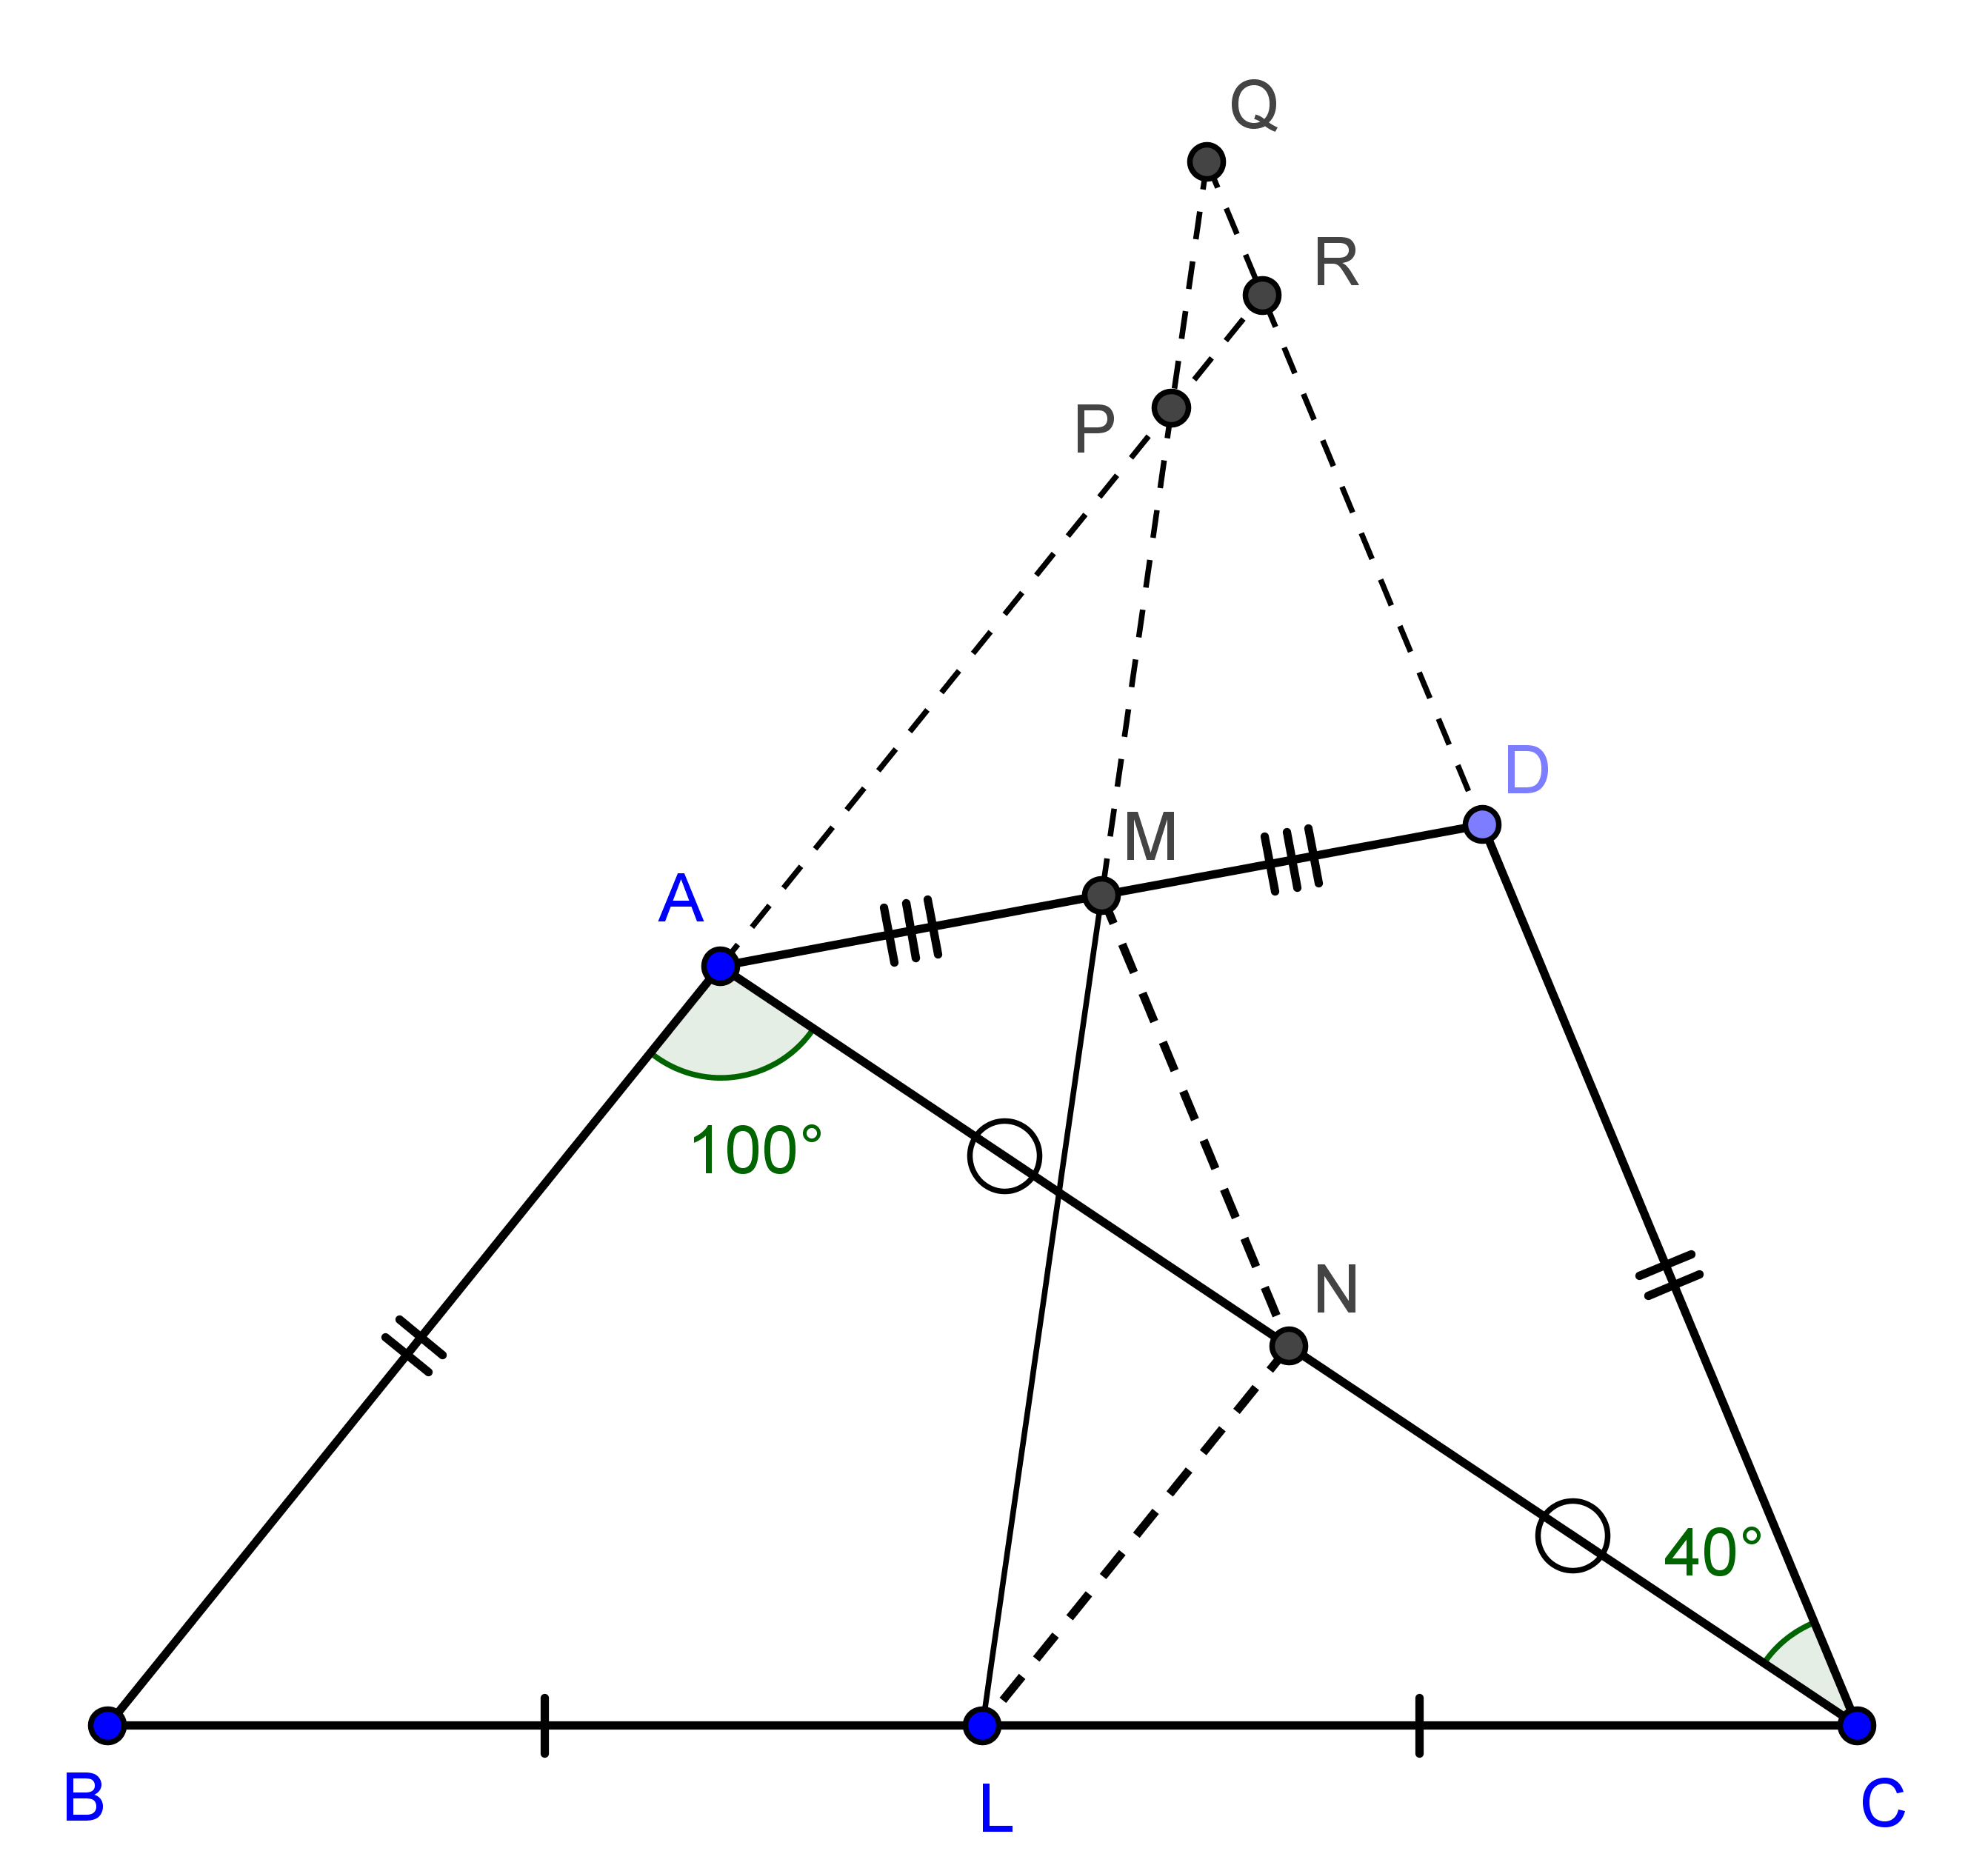
\includegraphics[width=0.5\textwidth]{advanced_geometry_67}
\ep

\bp
\(AM=BM=4\), \(PC=5\)일 때, \(\triangle BDP\)의 넓이를 구하여라.
\par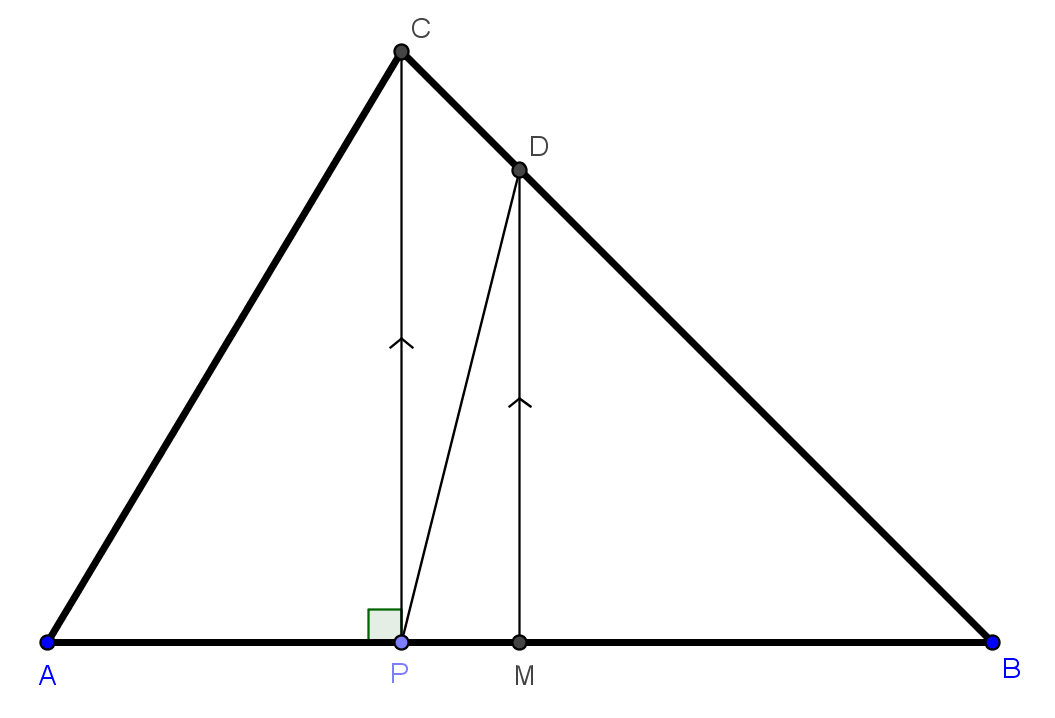
\includegraphics[width=0.5\textwidth]{advanced_geometry_69}
\ep
\end{document}